\chapter{Resultado}

\section{Avaliação W3C dos portais de transparência}

Para avaliar e quantificar a transparência das escolas municipais, foram utilizados os critérios de melhores práticas propostos pelo W3C \cite{W3C}. O W3C pontua 35 melhores práticas \cite{W3CSUMMARY} que podem ser seguidas para se alcançar uma boa padronização dos dados disponibilizados. A avaliação inicial se deu com os dados fornecidos pelo Programa de Transferência de Recursos Financeiros (PTRF) \cite{SP}, da Secretaria de Educação do Município de São Paulo, disponibilizado através dos dados abertos do Portal de Transparência. O resultado pode ser visualizado na tabela a seguir. No gráfico subsequente à tabela, é possível avaliar os valores de forma proporcional.

\begin{center}
\begin{tabularx}{1\textwidth} { 
  | >{\centering\arraybackslash}X 
  | >{\centering\arraybackslash}X | }
 \hline
 Boas Práticas W3C & Atende o Requisito \\
 \hline
 Fornecer Metadados & Sim \\
 \hline
 Fornecer metadados descritivos & Não \\
\hline
Fornecer metadados estruturais & Não \\
\hline
Fornecer Informações sobre a licença de dados & Sim \\
\hline
Fornecer informações sobre a procedência dos dados & Não \\
\hline
Fornecer informações de qualidade de dados & Não \\
\hline
Fornecer indicador de versão & Não \\
\hline
Fornecer o histórico de versão & Não se aplica \\
\hline
Usar URIs persistentes como identificadores de conjuntos de dados & Não \\
\hline
Usar URIs persistentes como identificadores dentro de conjunto de dados & Não \\
\hline
Atribuir URIs para as versões dos conjuntos de dados e séries & Não \\
\hline
Usar formatos de dados padronizados legíveis por máquinas & Sim \\
\hline
Usar reprentações de dados que sejam independentes de localidade & Sim \\
\hline
Fornecer dados em formatos múltiplos & Não \\
\hline
Reutilizar vocabulários, dando preferência aos padronizados & Sim \\
\hline
Escolher o nível de formalização adequado & Não se aplica \\
\hline
Fornecer download em massa & Sim \\
\hline
Fornecer subconjuntos para conjuntos de dados extensos & Não \\
\hline
Usar negociação de conteúdo para disponibilizar dados em formatos múltiplos & Não se aplica \\
\hline
Fornecer acesso em tempo real & Sim \\
\hline
Fornecer dados atualizados & Sim \\
\hline
Fornecer uma explicação para os dados que não estão disponíveis & Não se aplica \\
\hline
\end{tabularx}
\end{center}

\begin{center}
\begin{tabularx}{1\textwidth} { 
  | >{\centering\arraybackslash}X 
  | >{\centering\arraybackslash}X | }
  \hline
Disponibilizar dados por meio de uma API & Não \\
\hline
Usar padrões Web como base para construção de APIs & Não se aplica \\
\hline
Fornecer documentação completa para as APIs & Não se aplica \\
\hline
Evitar alterações que afetem o funcionamento de sua API & Não se aplica \\
\hline
Preservar identificadores & Sim \\
\hline
Avaliar a cobertura do conjunto de dados & Sim \\
\hline
Coletar feedback de consumidores de dados & Não \\
\hline
Compartilhar o feedback disponível & Não se aplica \\
\hline
Enriquecer dados por meio da geração de novos dados & Não \\
\hline
Fornecer visualizações complementares & Não \\
\hline
Fornecer feedback para o publicador original & Não se aplica \\
\hline
Obedecer os termos de licença & Sim \\
\hline
Citar a publicação original do conjunto de dados & Não \\
\hline
  \end{tabularx}
\end{center}

\begin{figure}[H]
    \centering
    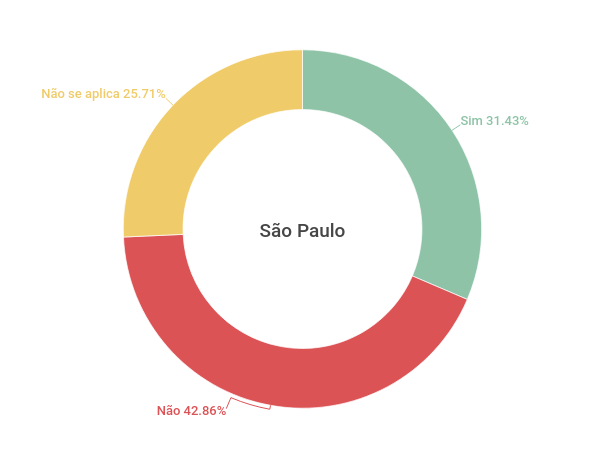
\includegraphics[scale=0.5]{images/grafico1.png}
    \label{fig:2}
\end{figure}

A análise dos dados do Programa de Transferência de Recursos Financeiros revelou que 31,43\% das boas práticas propostas para dados abertos são seguidas pela plataforma, sendo 25,71\% não aplicáveis e 42,86\% não cumpridas.

No entanto, esta é uma avaliação específica de um único município do país. Com esses pontos isolados, é difícil afirmar se a proporcionalidade está dentro do esperado. Por isso, a fim de quantificar a eficácia dos dados disponibilizados, avaliamos a disponibilidade de dados relativos à educação em outros municípios. É importante salientar que o programa PTRF é exclusivo do município de São Paulo, não existindo em outras cidades. Realizamos uma análise preliminar em diversas capitais municipais brasileiras e constatamos que, além da forma de disponibilização ser muito diferente, alguns sistemas apresentam falhas de funcionalidade. Com isso em mente, selecionamos quatro capitais específicas, uma para cada região do Brasil (desconsiderando o município de São Paulo da região Sudeste): Curitiba (Sul), Campo Grande (Centro-Oeste), Salvador (Nordeste) e Manaus (Norte).

Para cada município, extraiu-se ou avaliou-se os dados exibidos relativos às escolas municipais e à educação, utilizando as métricas do W3C como base. A planilha com a avaliação completa está disponível no Github \cite{GitHub}, sob o nome ``boasPraticas.odt''.

A seguir, destacamos a pontuação obtida por cada município em cada categoria. Abaixo, apresentamos os gráficos da pontuação de cada cidade.

\begin{figure}[H]
    \centering
    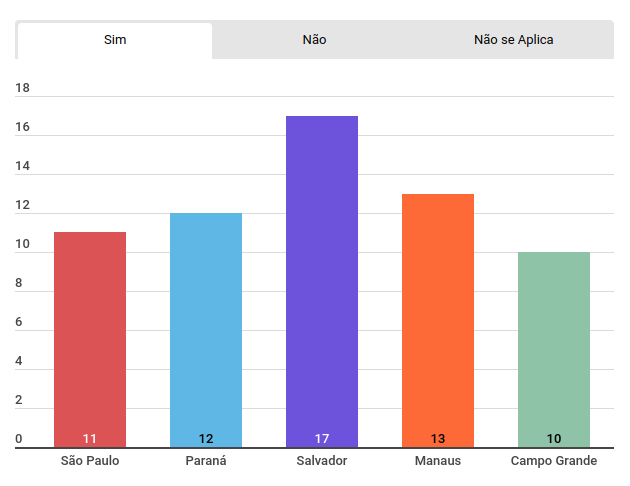
\includegraphics[scale=0.5]{images/grafico2.png}
    \label{fig:3}
\end{figure}

\begin{figure}[H]
    \centering
    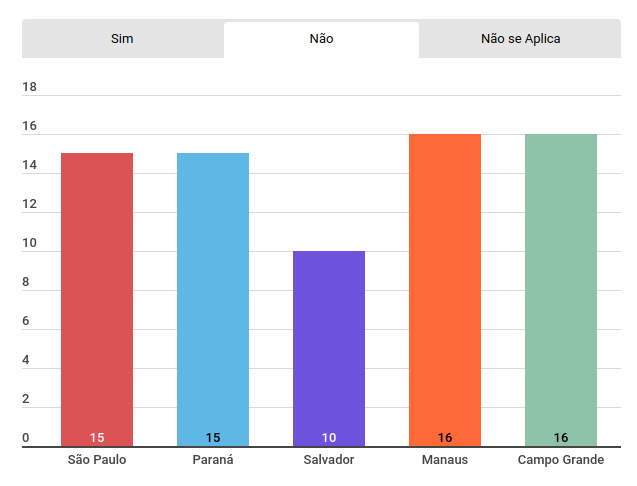
\includegraphics[scale=0.5]{images/grafico3.png}
    \label{fig:4}
\end{figure}

\begin{figure}[H]
    \centering
    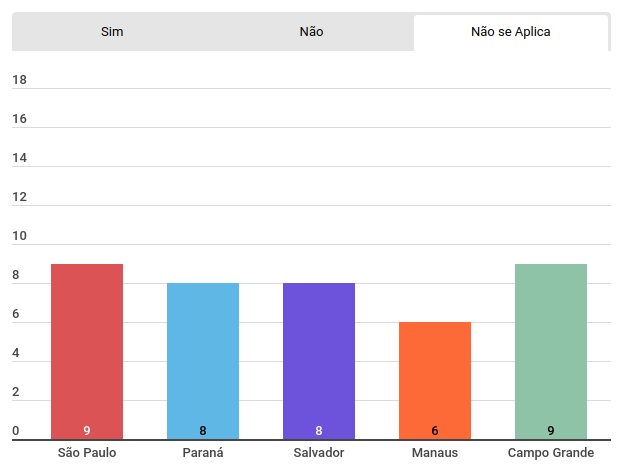
\includegraphics[scale=0.5]{images/grafico4.png}
    \label{fig:5}
\end{figure}

Os gráficos apresentados evidenciam que o município de São Paulo não demonstra um bom desempenho em transparência quando comparado a outras capitais brasileiras, pois está em quarto lugar na pontuação de ``Sim'', atrás de Paraná, Manaus e Salvador, sendo que este último atende a quase 50\% dos 35 requisitos. Em relação à classificação ``Não'', São Paulo tende a ficar na média das outras cidades.

Vale ressaltar algumas características observadas ao avaliar os portais de transparência. A primeira delas é que, além destes cinco municípios, os dados abertos das principais capitais sempre atendem a alguns pontos específicos do W3C: fornecimento de acesso em tempo real, fornecimento de dados atualizados e representação de dados que sejam independentes de localidade.

Acredita-se que esses pontos sempre serão atendidos (ou é esperado que sejam) devido a uma das principais leis que regulam a acessibilidade dos dados governamentais, a Lei Nº 12.527, conhecida como Lei de Transparência. Nesta lei, é especificado que os dados devem ser exibidos em tempo real (Art. 8, Inciso 4º), de forma atualizada (Art. 8, Inciso 3º) e em linguagem de fácil compreensão (Art. 5º).

Outra característica notada é que a disponibilização de dados por meio de API não era atendida em nenhum portal de transparência, inclusive nos cinco avaliados acima. Como consequência, os pontos de fornecimento de documentação completa da API, evitar alterações que afetem o funcionamento da API e usar padrões web como base para construção de API são considerados não aplicáveis.

Acreditamos que, por ser a API uma abordagem mais técnica de disponibilização de dados, essa implementação pode não ser tão conhecida para leigos, como arquivos nos formatos .CSV, .XLSX e outros. Essa pode ser uma explicação plausível para a ausência de dados disponíveis por meio de uma API.

